Selezionando nel menu \emph{Configurazione FreeTure} si accede alla sezione corrispondente dove è possibile modificare la definizione della configurazione del software per il rilevamento di meteore (cfr. figura \ref{fig:freeture}).
Nel dettaglio, si sono dovute realizzare tre sottosezioni differenti:
\begin{enumerate}[noitemsep,nolistsep]
    \item Caricamento di file di configurazione o di maschera
    \item Configurazione automatica
    \item Configurazione manuale
\end{enumerate}

\begin{figure}
    \begin{center}
    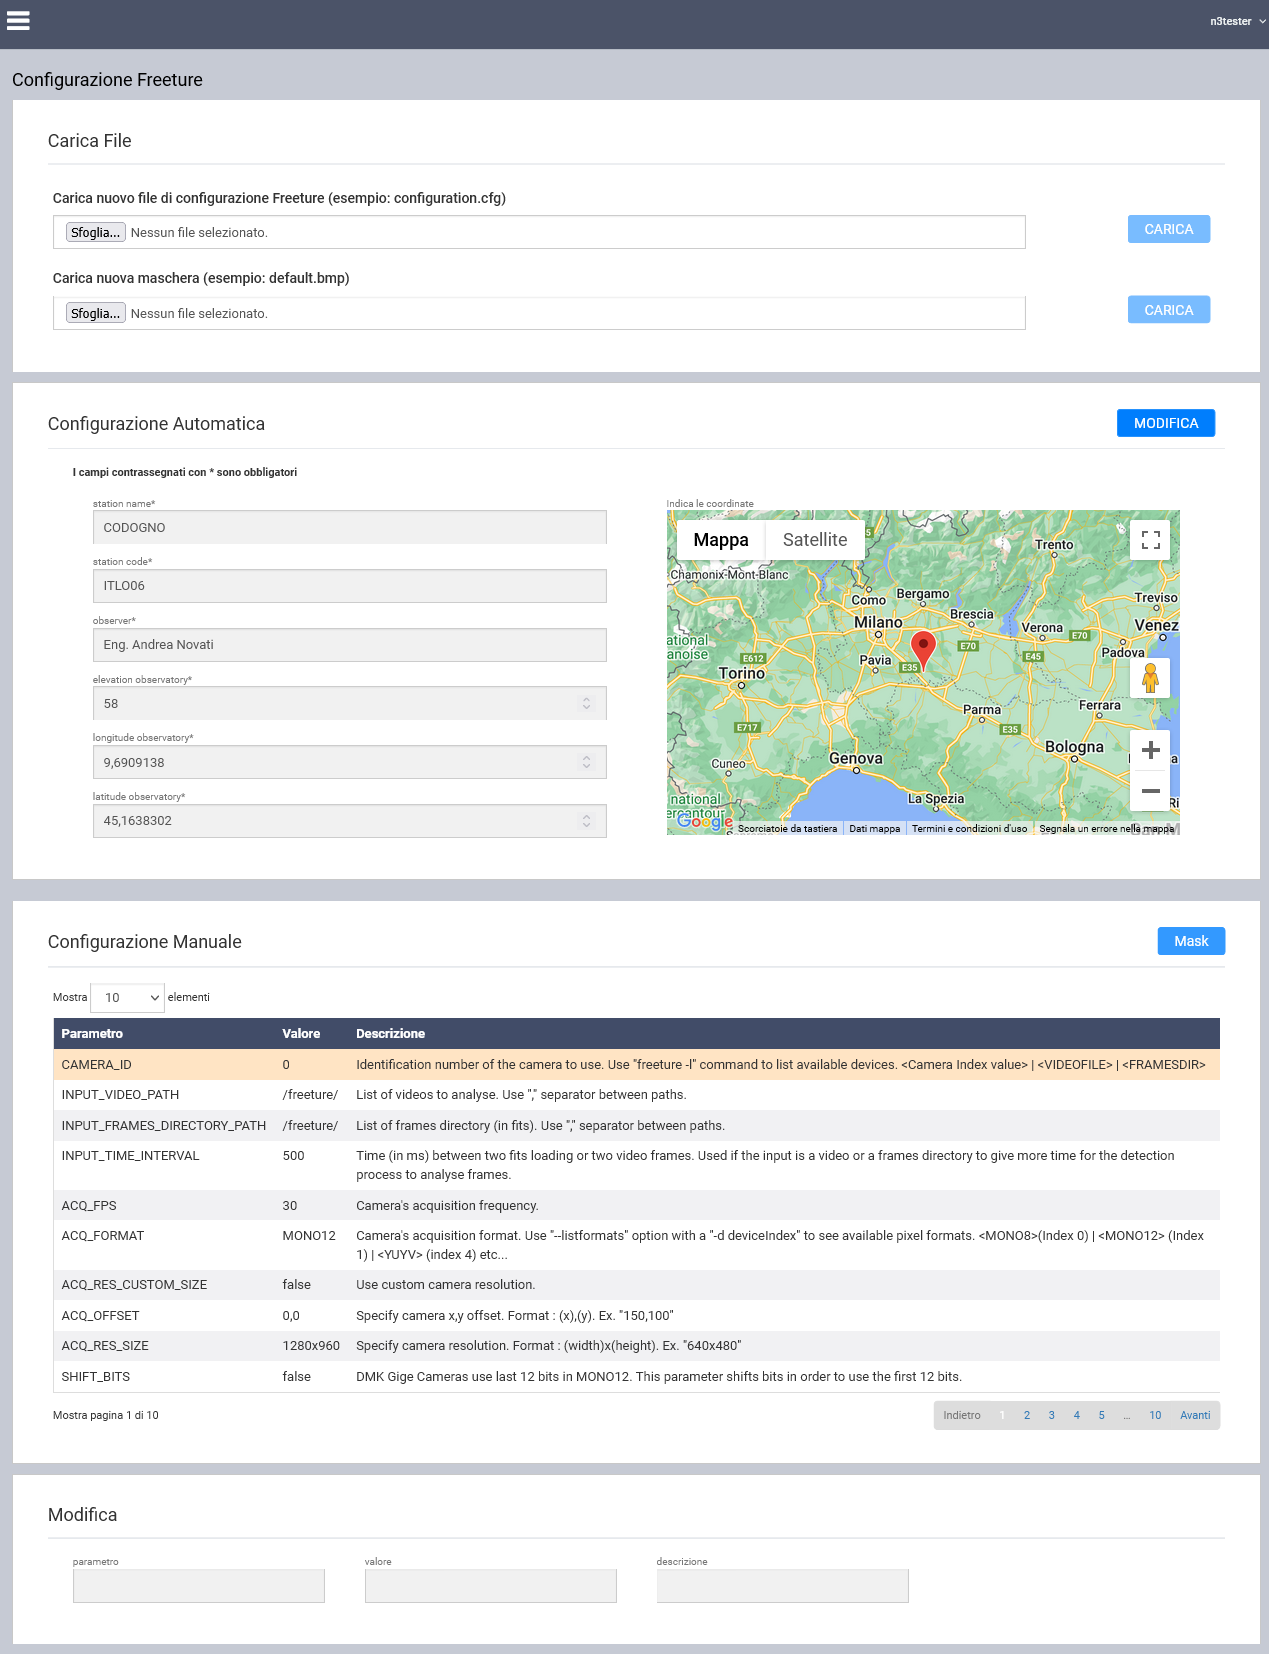
\includegraphics[width=\textwidth]{images/full-freeture.png}
    \caption{Sezione \emph{Configurazione FreeTure}.}
    \label{fig:freeture}
    \end{center}
\end{figure}

\subsection{Caricamento nuova configurazione}

Si permette all'utente di caricare un file di \textbf{configurazione} completo di FreeTure, in formato \textbf{CONF}, mediante un apposito \textbf{\emph{file picker}}. Il server, una volta ricevuto il file, lo copia nel rispettivo volume \emph{freeture-conf} e riavvia il container (cfr. sezione \ref{docker}).

L'utente può anche decidere di caricare una \textbf{maschera} (cfr. sezione \ref{freeture}) in formato \textbf{BMP}, sempre tramite file picker. In questo caso, il server copierà la maschera nel volume \emph{freeture-data} (cfr. sezione \ref{docker}), opzionalmente modificando il file di configurazione esistente per selezionare la presenza di una nuova maschera.

Un messaggio di successo è mostrato se le operazioni sono andate a buon fine.

\begin{figure}[H]
    \begin{center}
    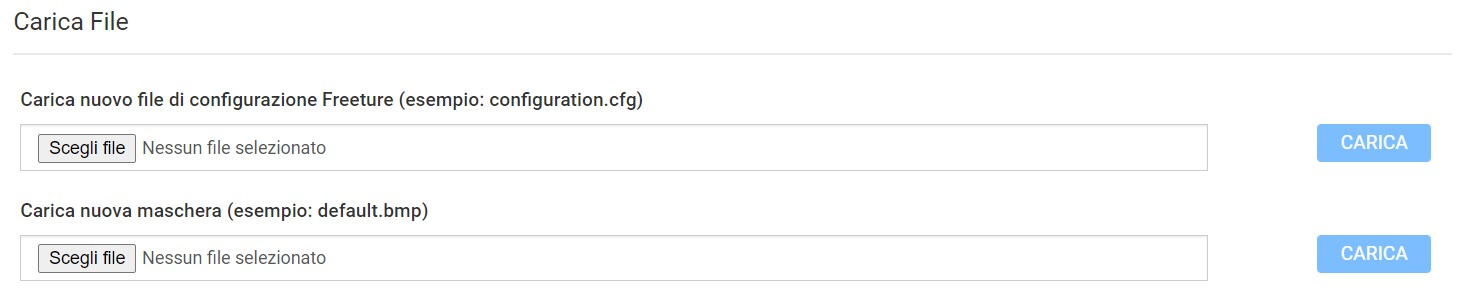
\includegraphics[width=\textwidth]{images/ft-carica-file.jpg}
    \caption{Caricamento file di configurazione o maschera.}
    \end{center}
\end{figure}

\subsection{Configurazione manuale}

Viene data la possibilità all'utente di modificare qualsiasi campo della configurazione; pertanto viene effettuato il parsing della configurazione dal server e visualizzato lato client con una tabella, realizzata tramite DataTables (cfr. sezione \ref{software}), le cui righe contengono \textbf{parametro}, \textbf{valore} e \textbf{descrizione} di ogni campo. Una volta cliccato sulla riga corrispondente, l'utente può modificare il valore del campo selezionato.
Un messaggio di successo è mostrato se l'operazione è andata a buon fine.

\begin{figure}[H]
    \begin{center}
    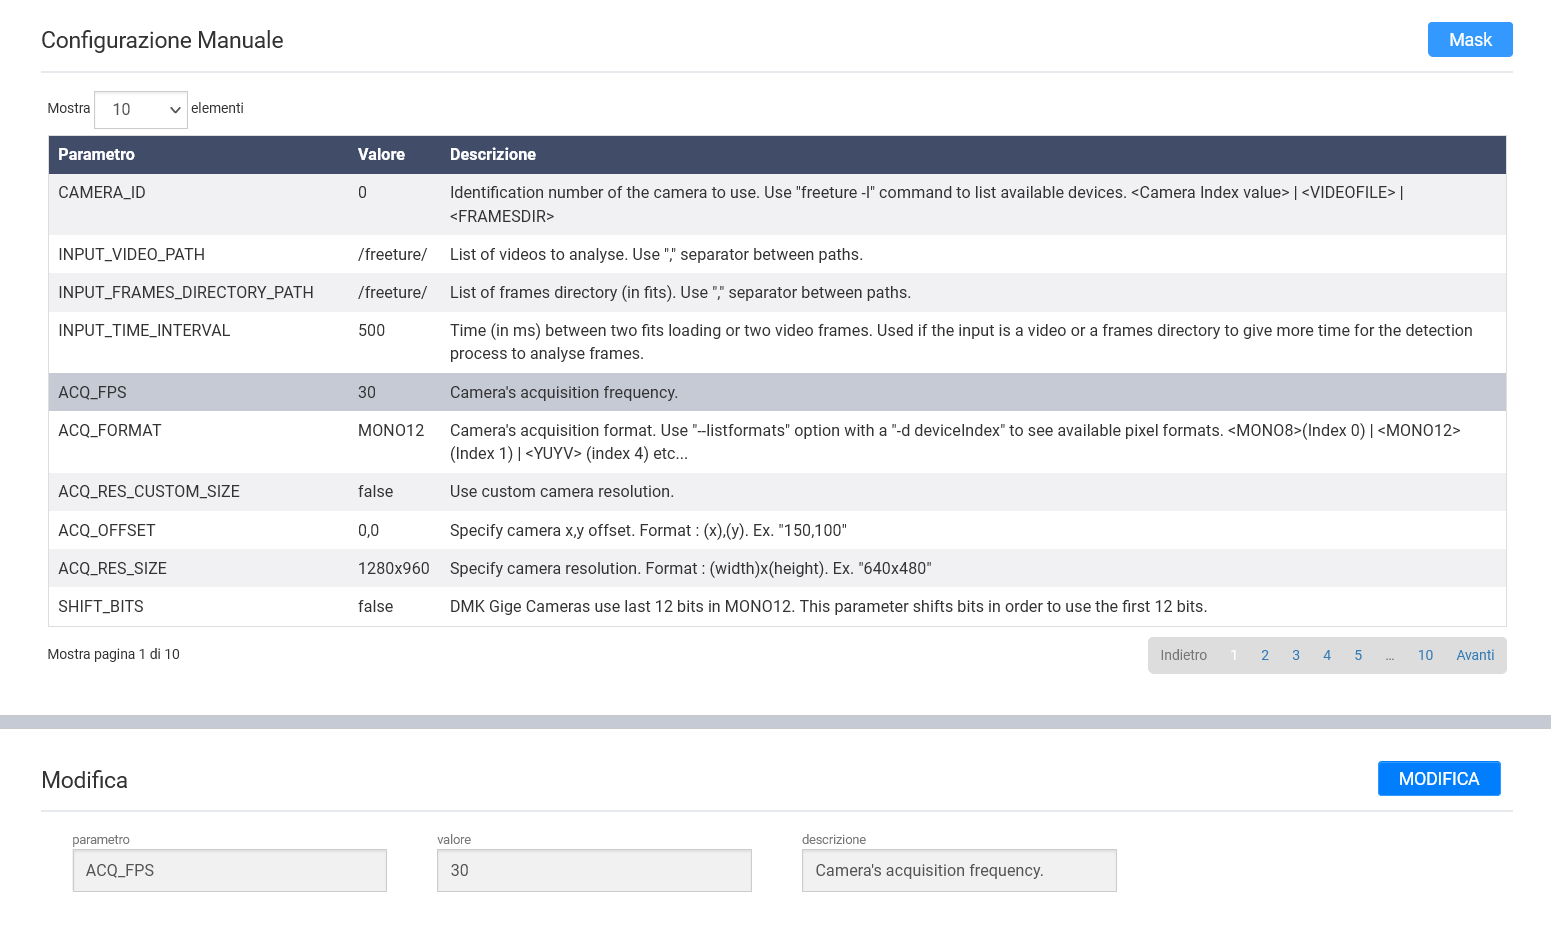
\includegraphics[width=\textwidth]{images/conf-manuale.png}
    \caption{Sezione di configurazione manuale. Sopra la tabella e sotto il campo di modifica del valore.}
    \end{center}
\end{figure}

\subsection{Configurazione automatica} \label{ft-conf-automatica}

Siccome, nella maggior parte dei casi, i principali campi oggetto di modifica sono ricorrenti e la modifica di un valore non è circoscritta ad un solo campo, l'utente può accedere ad una sezione di configurazione automatica, dove può modificare alcuni \textbf{valori chiave}. Le integrazioni a questi valori si ripercuotono poi su tutta la configurazione, andando a cambiare tutti i campi che sono coinvolti.

Una volta che la pagina web viene caricata, i campi in questione sono già precompilati con i valori correnti e l'utente può andare a cambiare solo quelli di suo interesse.

I campi sopracitati sono i seguenti:
\begin{itemize}
    \item \textbf{Nome della stazione}: solitamente è il nome della città dove si trova la stazione. È legato principalmente ai prefissi dei nomi dei file prodotti dalle elaborazioni astronomiche.
    \item \textbf{Codice della stazione}: è il codice univoco con cui si identifica la stazione. È coinvolto principalmente nei nomi delle cartelle generate da FreeTure.
    \item \textbf{Observer}: anagrafica della persona che gestisce la stazione.
    \item \textbf{Elevation observatory}: altitudine della stazione.
    \item \textbf{Longitude observatory}: longitudine della stazione.
    \item \textbf{Latitude observatory}: latitudine della stazione.
\end{itemize}

La web app si serve di un \textbf{sistema di validazione} dei campi degli input di tipo testo e numerico: all'utente non è ad esempio permesso lasciare un valore nullo. 

\begin{figure}[H]
    \begin{center}
    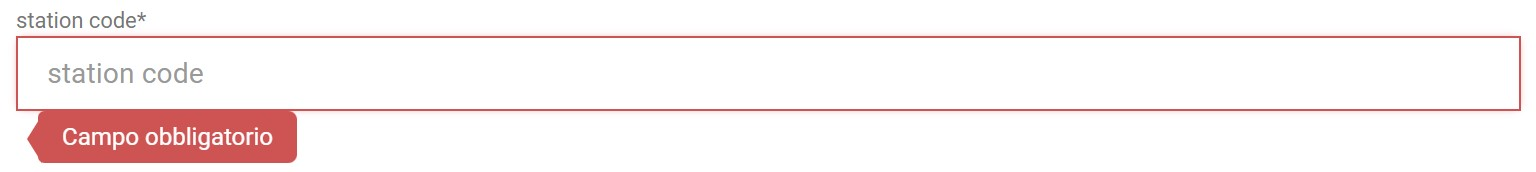
\includegraphics[width=\textwidth]{images/validator.jpg}
    \caption{Esempio di input improprio segnalato con un messaggio di errore.}
    \end{center}
\end{figure}

Inoltre, tramite l'utilizzo delle API di \textbf{GoogleMaps} (cfr. sezione \ref{software}), è stato realizzato un \textbf{\emph{location picker}}, grazie a cui l'utente può interagire con la mappa cliccando nel punto dove desidera localizzare la stazione, oppure avere un riscontro diretto dell'ubicazione delle coordinate inserite manualmente.

\begin{lstlisting}[style=JavaScript,caption={Parte dell'implementazione in JS per il \emph{location picker}.},captionpos=b,label={lst:location-picker}]
// Handle location picking
function changeMarkerLocation() {
    lat = Number($('#latitude-observatory').val());
    lng = Number($('#longitude-observatory').val());
    station = {lat: lat, lng: lng};
    if (marker === false) {
        marker = new google.maps.Marker({
            position: station,
            map: map,
            draggable: true
        });
        google.maps.event.addListener(marker, 'dragend', 
            function (event) {
                markerLocation();
            });
    } else {
        marker.setPosition(station);
    }
    map.setCenter({lat: lat, lng: lng});
}
\end{lstlisting}

\begin{figure}[H]
    \begin{center}
    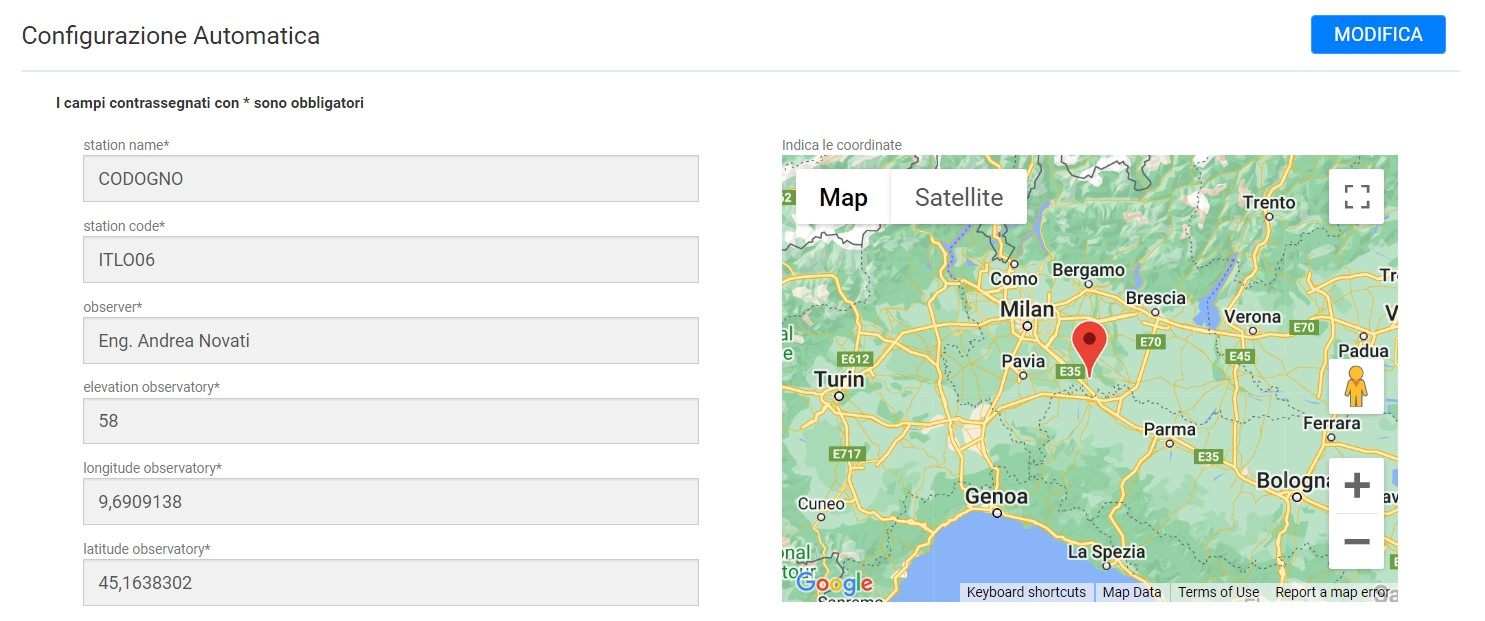
\includegraphics[width=\textwidth]{images/conf-automatica.jpg}
    \caption{Sezione di configurazione automatica. A destra il \emph{location picker} e a sinistra il campo di modifica del valore.}
    \end{center}
\end{figure}